\documentclass{article}

\usepackage[utf8]{inputenc}
\usepackage[T1]{fontenc}
\usepackage{amsmath}
\usepackage[framed]{matlab-prettifier}
%\usepackage[a4paper, total={6in, 8in}]{geometry}
\usepackage[a4paper, margin=4cm,top=2cm,landscape]{geometry}
\usepackage[italian]{babel}
\usepackage{pdfpages}


\setlength{\parskip}{5pt}
\setlength{\parindent}{0pt}
\lstset{
style      = Matlab-editor,
basicstyle = \mlttfamily,
%backgroundcolor = \color{lightgray},
numbers=left,
numbersep=5pt,
numberstyle=\tiny\color{gray},
tabsize=2,
morekeywords={yyaxis,abs,logspace,loglog,xlabel,ylabel,figure,exp,title,semilogx,legend,zeros,rand,ones,tic,toc,plot},
frameshape={RYR}{Y}{Y}{RYR},
}


\begin{document}
	\begin{lstlisting}
	format long
	N = 50;
	volte = 1;
	voltetot = 100;
	res = zeros(voltetot,1);
	while volte < voltetot
	A = rand(N);
	%if (rank(A)==N) & (cond(A) < 500)
	%sprintf("rank(A): %3f, cond(A): %3f",rank(A),cond(A))
	command = "./a.out " + num2str(N);
	for i=1:N
	for j=1:N
	command = command + " " + num2str(A(i,j),20);
	end
	end
	[status,cmdout] = system(command);
	xC = str2num(cmdout)';
	xVera = A\ones(N,1);
	res(volte) = norm(xVera-xC)/norm(xVera);
	volte = volte+1;
	%end
	end
	figure();
	semilogy(res,'o','MarkerSize',15);
	title('Errore Relativo soluzione sistema lineare C vs MATLAB');
	xlabel('Varie Esecuzioni con input casuali');
	ylabel('Errore Relativo');
	\end{lstlisting}
	
	\includepdf{./img.eps}
\end{document}